\section{Verdikonfigurasjons-analyse}
Verdikonfigurasjonsanalysen identifiserer sammensetningen av bedriftens aktiviteter og tilhørende verdi- og kostnadsdrivere (s. 32). AS ROCKWOOL driver med industriell produksjon som er typisk for en verdikjede.

\begin{figure}[H]
\centering
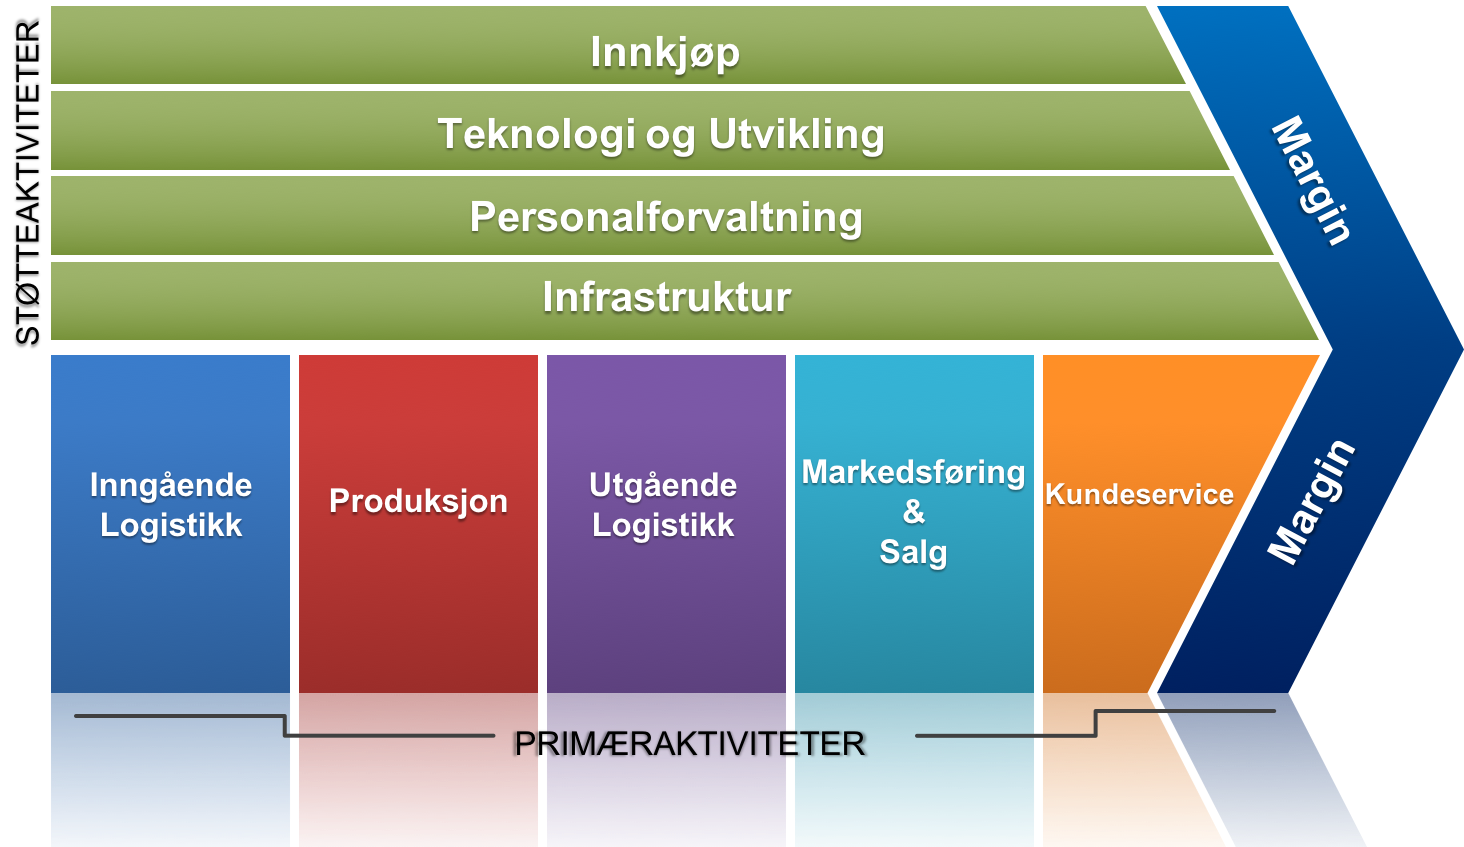
\includegraphics [scale=0.5]{bilder/verdikjede.png}
\caption{ROCKWOOL verdikjede}
\label{fig:verdikjede}
\end{figure}

\subsection{Primæraktiviteter}
Primæraktivitene er et sekvensielt sett av aktiviteter som direkte skaper verdi for kunden (s.132). 
 
\indent \newline
Som vist i figur \ref{fig:verdikjede} over er den første aktiviteten inngående logistikk. Råvarer som vulkansk stein, koks og slagg (avfallsprodukter fra aluminiumsproduksjon) lagres, før det fraktes videre til produksjon. Her omformes innsatsfaktorene fra råvarer til steinull ved å bli utsatt for enormt høye temperaturer i en smelteovn. De ferdige produktene fraktes videre til lagring eller transporteres direkte til kunder avhengig av om det er produsert på bestilling. Markedsføring og salg fokuserer på byggevarekjedene og entrepenørene. Det markedsføres derfor ikke direkte mot privatpersoner. Kundeservice består i hovedsak av teknisk service.
ROCKWOOL har utfordringer med høye transportkostnader i forhold til andre konkurrenter grunnet hvor godt produktene lar seg komprimere. Produktene transporteres med lastebil ved fastprisavtale, og dårligere komprimering av produktene gir lavere volum per transport. 

\subsection{Støtteaktiviteter}
Støtteaktivitetene skaper indirekte verdi for kunden gjennom sin effekt på primæraktivitetene (s.132). 

\subsubsection*{Innkjøp}
AS ROCKWOOL sin størrelse og del av konsern gir gjennom sentral koordinering og store innkjøpskvantum, fordelaktige innkjøpsavtaler.

\subsubsection*{Teknologi og utvikling}
Både i AS ROCKWOOL og konsernet har de i mange år lagt mye ressurser i teknologiutvikling. De har tidligere utviklet sitt eget bindemiddel som gir konkurransefortrinn i form av et produkt som har et større anvendelsesområde enn å bare isolere. I dag jobbes det med å utvikle produksjonsutstyr som kan bidra til å produsere et mer miljøvennlig produkt.

\subsubsection*{Personalforvaltning}
De ansatte trives godt i jobben og føler tilhørighet til arbeidsoppgavene. Det er innarbeidet gode rutiner som sørger for at det er to personer med samme kompetanse til å utføre hver arbeidsoppgave. Dette sørger for en kontinuerlig flyt selv ved sykefravær og eventuelle oppsigelser. 

\subsubsection*{Infrastruktur}
Vedlikehold og drift av produksjonen vurderes regelmessig etter KPI nøkkeltall som iverksetter . De større utstyr investeringer bærer preg av høye driftskostnader og overordnet startegi går på å nå måltall, markedsandeler, omsetning, vekst, bærekraft, digital platform, salgssystemer, produktutvikling, cost-saving

\indent \newline
ROCKWOOL har i dag to fabrikker lokalisert henholdsvis i Moss og Trondheim, og en administrasjon og salgsapparat i Oslo. En klar og overordnet visjon blir kommunisert godt gjennom alle avdelinger som sørger for en mest mulig effektiv drift. Må skrive noe annet også.
  
\subsubsection*{Oppsummering?}
AS ROCWOOL har i flere år jobbet med å effektivisere verdiekjeden. De har implementert en lean-metode som de kaller Ropex. (https://www.dagsavisen.no/moss/lokalt/viktig-for-industribyen-moss-1.316778).
Bedriften kjennetegnes derfor av god kommunikasjon på tvers av avdelinger og kommandolinjer med fokus på å produsere mest mulig effektivt. På bakgrunn av dette, ser man lite rom for forbedring i verdikjeden. ROCKWOOL bør imidlertid fortsette å investere i teknologiutvikling for å kunne forbedre kompaktheten til produktene og dermed øke volumet per transport.

\section{Verdikjedens drivere}
Dette er strukturelle faktorer som påvirker verdiskapning for kunden og enhetskostnadene forbundet med å utføre aktivitetene.(s.32) De viktigste driverne for AS ROCKWOOL er stordriftsfordeler og kapasitetsutnyttelse. Bedriften kan lagre produktene i opp til ett år før de må gjennom en ny kvalitetskontroll. Lang holdbarhet på produktene gir mulighet til å produsere i stor skala og dermed senke enhetskostnadene.

\indent \newline
Stordriftsfordelene forsterkes også av å være en del av ROCKWOOL-konsernet. Bedriften drar nytte av operasjonelle synergier gjennom gunstige prisavtaler hos leverandører ved å handle i stort kvantum.

\section{VRIO-analyse}
\begin{table}[ht]
\centering
\begin{tabular}{|>{\columncolor[HTML]{9B0000}}l |c|c|c|c|c|}
\hline
{\color[HTML]{FFFFFF} \textbf{Ressurs}} & \cellcolor[HTML]{656565}{\color[HTML]{FFFFFF} \textbf{Verdifull}} &  \cellcolor[HTML]{656565}{\color[HTML]{FFFFFF} \textbf{Sjelden}} & \cellcolor[HTML]{656565}{\color[HTML]{FFFFFF} \textbf{Vanskelig å kopiere}} & \cellcolor[HTML]{656565}{\color[HTML]{FFFFFF} \textbf{Effektivt organisert}} & \cellcolor[HTML]{656565}{\color[HTML]{FFFFFF} \textbf{Avkastning}} 
\\ \hline
{\color[HTML]{FFFFFF} \textbf{Finansiell kapital}} & \cmark & \xmark & \xmark & \cmark & Over gjennomsnittet                                                \\ \hline
{\color[HTML]{FFFFFF} \textbf{Kompetanse}} & \cmark & \cmark & \cmark & \cmark & Over gjennomsnittet                                                \\ \hline
{\color[HTML]{FFFFFF} \textbf{Teknologi}} & \cmark  & \xmark & \xmark & \xmark & Litt under gjennomsnittet 
\\ \hline
{\color[HTML]{FFFFFF} \textbf{Produktegenskaper}}  & \cmark & \xmark  & \cmark & \cmark & Over gjennomsnittet                                                \\ \hline
\end{tabular}
\caption{My caption}
\label{my-label}
\end{table}

\subsection{Finansiell kapital}
AS ROCKWOOL har hatt en lønnsom drift i flere år og hadde i 2017 et årsresultat på 64 millioner kr og en egenkapital på 382 millioner kr.(ref proff.no) I tillegg drar de nytte av finansielle synergier ved å være en del av et konsern. De står dermed godt rustet for potensielle investeringer i tiden fremover.

\subsection{Kompetanse}
Kompetansen anses som meget god. Turnover-raten er på bare 2% og mange av de ansatte har en fartstid på 15-35 år i bedriften. For å fortsette og utvikle kompetansen blant de ansatte, har de innarbeidet interne opplærings- og utdanningssystemer. Bedriften bør imidlertid være oppmerksom på at mye av kompetansen kan forsvinne i årene som kommer på grunn av en relativt høy gjennomsnittsalder hos de ansatte.

\subsection{Teknologi}
Det investeres mye ressurser i teknologi, både i AS ROCKWOOL og konsernet. Ved å utvikle egne smelteovner har dette tidligere gitt konkurransefortrinn i markedet, men med dagens smelteteknologi henger de etter de største konkurrentene når det gjelder å produsere miljøvennlig. Å redusere CO2-utslipp i forbindelse med produksjonsprosessen anses som kritisk for å kunne være konkurransedyktige i fremtiden.

\subsection{Produktegenskaper}
Steinull innehar flere egenskaper og bruksområder enn de fleste andre isolasjonsproduktene som tilbys i markedet. Produktet isolerer, er vannavstøtende, har lyddempende egenskaper og er en god kilde til brannsikring. Det er kun ROCKWOOL og Paroc som scorer høyt på alle disse produktatributtene, mens andre aktører kun leverer på to av punktene.  

\subsection{Oppsummering (sensorveiledning - gode oppgaver oppsummerer hvilke ressurser som gir konk.fortrinn - hva er viktig fremover?)}
Analysen viser at ROCKWOOL, sammen med Paroc, har konkurransefortrinn i produktegenskapene. Dette anses som langvarig da egenskapene kommer naturlig fra råvaren, og det vil også være kostbart for andre aktører å bytte til steinullproduksjon i form av store investeringer og mangel på erfaring. Det vil være viktig fremover å utvikle og/eller investere i ny miljøvennlig smelteteknologi . Dette anses som bedriftens største utfordring i dag.